\begin{figure}[htbp]
    \centering
    \begin{tikzpicture}[scale=1,x=1in,y=1in]
      \draw[white] (-2.0,-2.0) rectangle (2.0,2.0);
      \node {\pgftext{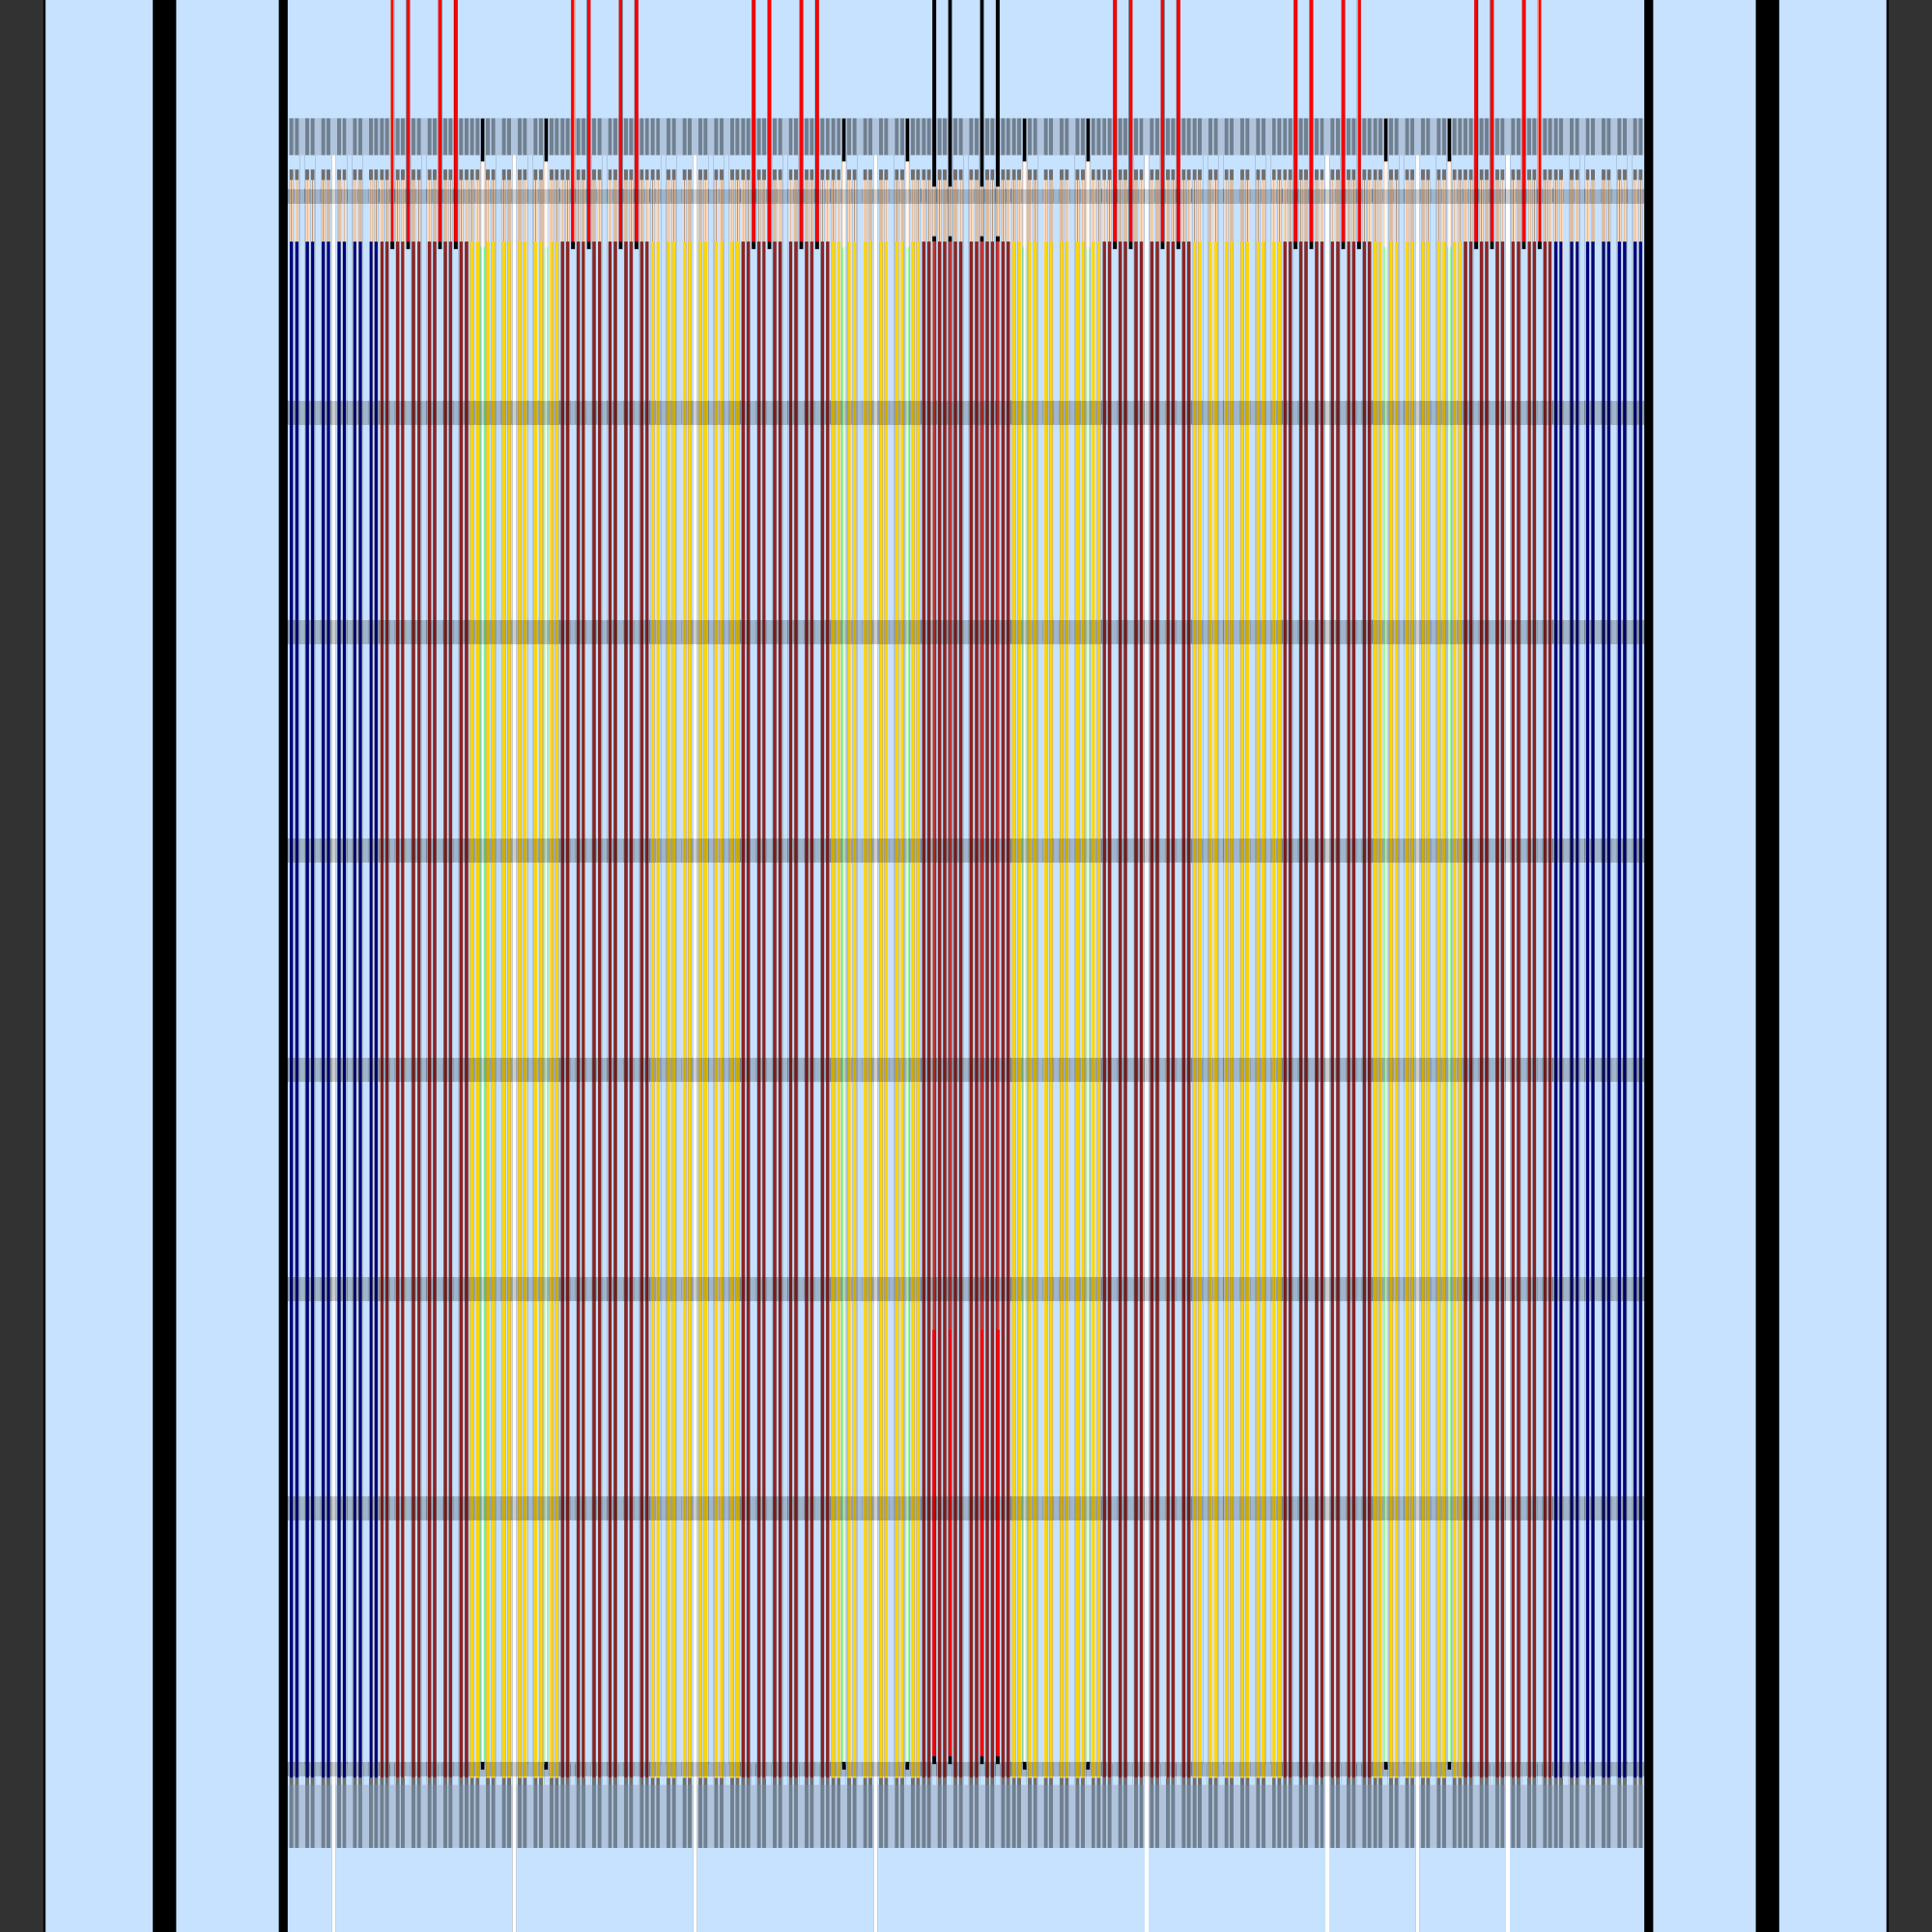
\includegraphics[width=4.0in]{specifications/axial/figs/row_8_mats_axial_grids_enhanced.png}}};
      \draw[red] (1.40241130435,-2.0) -- (2.2,-2.0) -- (2.4,-2.0) -- (2.55,-2.0) node[black,right,anchor=west,font=\scriptsize] {~0.00000 ~~~~~~~~ Lowest Extent};
      \draw[red] (1.40241130435,-1.82608695652) -- (2.2,-1.82608695652) -- (2.4,-1.88235294118) -- (2.55,-1.88235294118) node[black,right,anchor=west,font=\scriptsize] {~20.0000 ~~~~~~~~ Bottom of Support Plate};
      \draw[red] (1.40241130435,-1.69565217391) -- (2.2,-1.69565217391) -- (2.4,-1.76470588235) -- (2.55,-1.76470588235) node[black,right,anchor=west,font=\scriptsize] {~35.0000 ~~~~~~~~ Bottom of Fuel Rod};
      \draw[red] (1.40241130435,-1.68045217391) -- (2.2,-1.68045217391) -- (2.4,-1.64705882353) -- (2.55,-1.64705882353) node[black,right,anchor=west,font=\scriptsize] {~36.7480 ~~~~~~~~ Bottom of Active Fuel};
      \draw[red] (1.40241130435,-1.67685130435) -- (2.2,-1.67685130435) -- (2.4,-1.52941176471) -- (2.55,-1.52941176471) node[black,right,anchor=west,font=\scriptsize] {~37.1621 ~~~~~~~~ Grid 1 Bottom};
      \draw[red] (1.40241130435,-1.66382608696) -- (2.2,-1.66382608696) -- (2.4,-1.41176470588) -- (2.55,-1.41176470588) node[black,right,anchor=west,font=\scriptsize] {~38.6600 ~~~~~~~~ Bot. of BPRA Rod};
      \draw[red] (1.40241130435,-1.65253913043) -- (2.2,-1.65253913043) -- (2.4,-1.29411764706) -- (2.55,-1.29411764706) node[black,right,anchor=west,font=\scriptsize] {~39.9580 ~~~~~~~~ Control Rod Step 0};
      \draw[red] (1.40241130435,-1.64765217391) -- (2.2,-1.64765217391) -- (2.4,-1.17647058824) -- (2.55,-1.17647058824) node[black,right,anchor=west,font=\scriptsize] {~40.5200 ~~~~~~~~ Grid 1 Top};
      \draw[red] (1.40241130435,-1.64732173913) -- (2.2,-1.64732173913) -- (2.4,-1.05882352941) -- (2.55,-1.05882352941) node[black,right,anchor=west,font=\scriptsize] {~40.5580 ~~~~~~~~ Bottom of Active Absorber};
      \draw[red] (1.40241130435,-1.63627826087) -- (2.2,-1.63627826087) -- (2.4,-0.941176470588) -- (2.55,-0.941176470588) node[black,right,anchor=west,font=\scriptsize] {~41.8280 ~~~~~~~~ Bottom of Lower Absorber (AIC)};
      \draw[red] (1.40241130435,-1.14760869565) -- (2.2,-1.14760869565) -- (2.4,-0.823529411765) -- (2.55,-0.823529411765) node[black,right,anchor=west,font=\scriptsize] {~98.0250 ~~~~~~~~ Grid 2 Bottom};
      \draw[red] (1.40241130435,-1.09791304348) -- (2.2,-1.09791304348) -- (2.4,-0.705882352941) -- (2.55,-0.705882352941) node[black,right,anchor=west,font=\scriptsize] {~103.740 ~~~~~~~~ Grid 2 Top};
      \draw[red] (1.40241130435,-0.69372173913) -- (2.2,-0.69372173913) -- (2.4,-0.588235294118) -- (2.55,-0.588235294118) node[black,right,anchor=west,font=\scriptsize] {~150.222 ~~~~~~~~ Grid 3 Bottom};
      \draw[red] (1.40241130435,-0.644026086957) -- (2.2,-0.644026086957) -- (2.4,-0.470588235294) -- (2.55,-0.470588235294) node[black,right,anchor=west,font=\scriptsize] {~155.937 ~~~~~~~~ Grid 3 Top};
      \draw[red] (1.40241130435,-0.239834782609) -- (2.2,-0.239834782609) -- (2.4,-0.352941176471) -- (2.55,-0.352941176471) node[black,right,anchor=west,font=\scriptsize] {~202.419 ~~~~~~~~ Grid 4 Bottom};
      \draw[red] (1.40241130435,-0.190139130435) -- (2.2,-0.190139130435) -- (2.4,-0.235294117647) -- (2.55,-0.235294117647) node[black,right,anchor=west,font=\scriptsize] {~208.134 ~~~~~~~~ Grid 4 Top};
      \draw[red] (1.40241130435,0.214052173913) -- (2.2,0.214052173913) -- (2.4,-0.117647058824) -- (2.55,-0.117647058824) node[black,right,anchor=west,font=\scriptsize] {~254.616 ~~~~~~~~ Grid 5 Bottom};
      \draw[red] (1.40241130435,0.263747826087) -- (2.2,0.263747826087) -- (2.4,0.0) -- (2.55,0.0) node[black,right,anchor=west,font=\scriptsize] {~260.331 ~~~~~~~~ Grid 5 Top};
      \draw[red] (1.40241130435,0.667939130435) -- (2.2,0.667939130435) -- (2.4,0.117647058824) -- (2.55,0.117647058824) node[black,right,anchor=west,font=\scriptsize] {~306.813 ~~~~~~~~ Grid 6 Bottom};
      \draw[red] (1.40241130435,0.717634782609) -- (2.2,0.717634782609) -- (2.4,0.235294117647) -- (2.55,0.235294117647) node[black,right,anchor=west,font=\scriptsize] {~312.528 ~~~~~~~~ Grid 6 Top};
      \draw[red] (1.40241130435,1.12182608696) -- (2.2,1.12182608696) -- (2.4,0.352941176471) -- (2.55,0.352941176471) node[black,right,anchor=west,font=\scriptsize] {~359.010 ~~~~~~~~ Grid 7 Bottom};
      \draw[red] (1.40241130435,1.17152173913) -- (2.2,1.17152173913) -- (2.4,0.470588235294) -- (2.55,0.470588235294) node[black,right,anchor=west,font=\scriptsize] {~364.725 ~~~~~~~~ Grid 7 Top};
      \draw[red] (1.40241130435,1.48380869565) -- (2.2,1.48380869565) -- (2.4,0.588235294118) -- (2.55,0.588235294118) node[black,right,anchor=west,font=\scriptsize] {~400.638 ~~~~~~~~ Control Rod Step 228};
      \draw[red] (1.40241130435,1.48902608696) -- (2.2,1.48902608696) -- (2.4,0.705882352941) -- (2.55,0.705882352941) node[black,right,anchor=west,font=\scriptsize] {~401.238 ~~~~~~~~ Top of Active Absorber};
      \draw[red] (1.40241130435,1.50006956522) -- (2.2,1.50006956522) -- (2.4,0.823529411765) -- (2.55,0.823529411765) node[black,right,anchor=west,font=\scriptsize] {~402.508 ~~~~~~~~ Top of Active Fuel};
      \draw[red] (1.40241130435,1.51111304348) -- (2.2,1.51111304348) -- (2.4,0.941176470588) -- (2.55,0.941176470588) node[black,right,anchor=west,font=\scriptsize] {~403.778 ~~~~~~~~ Bottom of Control Rod Plenum};
      \draw[red] (1.40241130435,1.58092173913) -- (2.2,1.58092173913) -- (2.4,1.05882352941) -- (2.55,1.05882352941) node[black,right,anchor=west,font=\scriptsize] {~411.806 ~~~~~~~~ Grid 8 Bottom};
      \draw[red] (1.40241130435,1.61012173913) -- (2.2,1.61012173913) -- (2.4,1.17647058824) -- (2.55,1.17647058824) node[black,right,anchor=west,font=\scriptsize] {~415.164 ~~~~~~~~ Grid 8 Top};
      \draw[red] (1.40241130435,1.61354782609) -- (2.2,1.61354782609) -- (2.4,1.29411764706) -- (2.55,1.29411764706) node[black,right,anchor=west,font=\scriptsize] {~415.558 ~~~~~~~~ Top of Control Rod Plenum};
      \draw[red] (1.40241130435,1.62751304348) -- (2.2,1.62751304348) -- (2.4,1.41176470588) -- (2.55,1.41176470588) node[black,right,anchor=west,font=\scriptsize] {~417.164 ~~~~~~~~ Top of Fuel Rod Plenum};
      \draw[red] (1.40241130435,1.6496) -- (2.2,1.6496) -- (2.4,1.52941176471) -- (2.55,1.52941176471) node[black,right,anchor=west,font=\scriptsize] {~419.704 ~~~~~~~~ Top of Fuel Rod};
      \draw[red] (1.40241130435,1.66549565217) -- (2.2,1.66549565217) -- (2.4,1.64705882353) -- (2.55,1.64705882353) node[black,right,anchor=west,font=\scriptsize] {~421.532 ~~~~~~~~ Top of BPRA Rod Plenum};
      \draw[red] (1.40241130435,1.67868695652) -- (2.2,1.67868695652) -- (2.4,1.76470588235) -- (2.55,1.76470588235) node[black,right,anchor=west,font=\scriptsize] {~423.049 ~~~~~~~~ Bottom of Upper Nozzle};
      \draw[red] (1.40241130435,1.75544347826) -- (2.2,1.75544347826) -- (2.4,1.88235294118) -- (2.55,1.88235294118) node[black,right,anchor=west,font=\scriptsize] {~431.876 ~~~~~~~~ Top of Upper Nozzle};
      \draw[red] (1.40241130435,2.0) -- (2.2,2.0) -- (2.4,2.0) -- (2.55,2.0) node[black,right,anchor=west,font=\scriptsize] {~460.000 ~~~~~~~~ Highest Extent};
      \draw (2.4,2.11764705882) node[left,anchor=west,font=\scriptsize] {\underline{Elevation (cm)} ~~~ \underline{Description}};

    \end{tikzpicture}


    \caption[Scale view of all axial planes.]{\emph{Left}: Scale view of row 8 axial cross section, with highlighted grid spacers and partial insertion of control rod bank D to the bite position. \emph{Right}: exhaustive list of all axial planes used in the model, excluding partial control rod insertion planes.\label{fig_all_axials}}
\end{figure}